\section{Theory: Neural dynamics}
\label{sec:NeuralDynamics}
\begin{itemize}
\item Multicompartmental modeling
\item Cable equation
\item No current monopoles - trick needed for point neurons
\end{itemize}

Modelling of neurons is at the core of computational neuroscience, and the topic has been treated in detail in several text books (see e.g., \cite{KockSegev1998, Koch1999, Hille2001, Dayan2005, Sterratt2011}). We therefore only give a brief introduction to it here. 

\subsection{Multicompartmental modeling}
Most simulations of extracellular potentials are based on multicompartmental neuronal models based on a Hodgkin-Huxley-type formalism. A model of a neuron is then characterized by (i) its morphology, and (ii) its membrane mechanisms. 

In a multicompartmental model, the morphology of the real neuron (Fig. \ref{fig:multicomp}A) is discretized as a set of compartments connected by resistors (Fig. \ref{fig:multicomp}B). In such a model there are two kinds of currents which together determine the membrane potential dynamics of the neuron (Fig. \ref{fig:multicomp}C). These are the currents that run intracellularly between compartments (yellow arrows), and the transmembrane currents (green arrows). Below, first present a framework for modeling the transmembrane currents in a single compartment, and next show how a number of such compartments can be connected together to a multicompartment model.

\begin{figure}[!ht]
\begin{center}
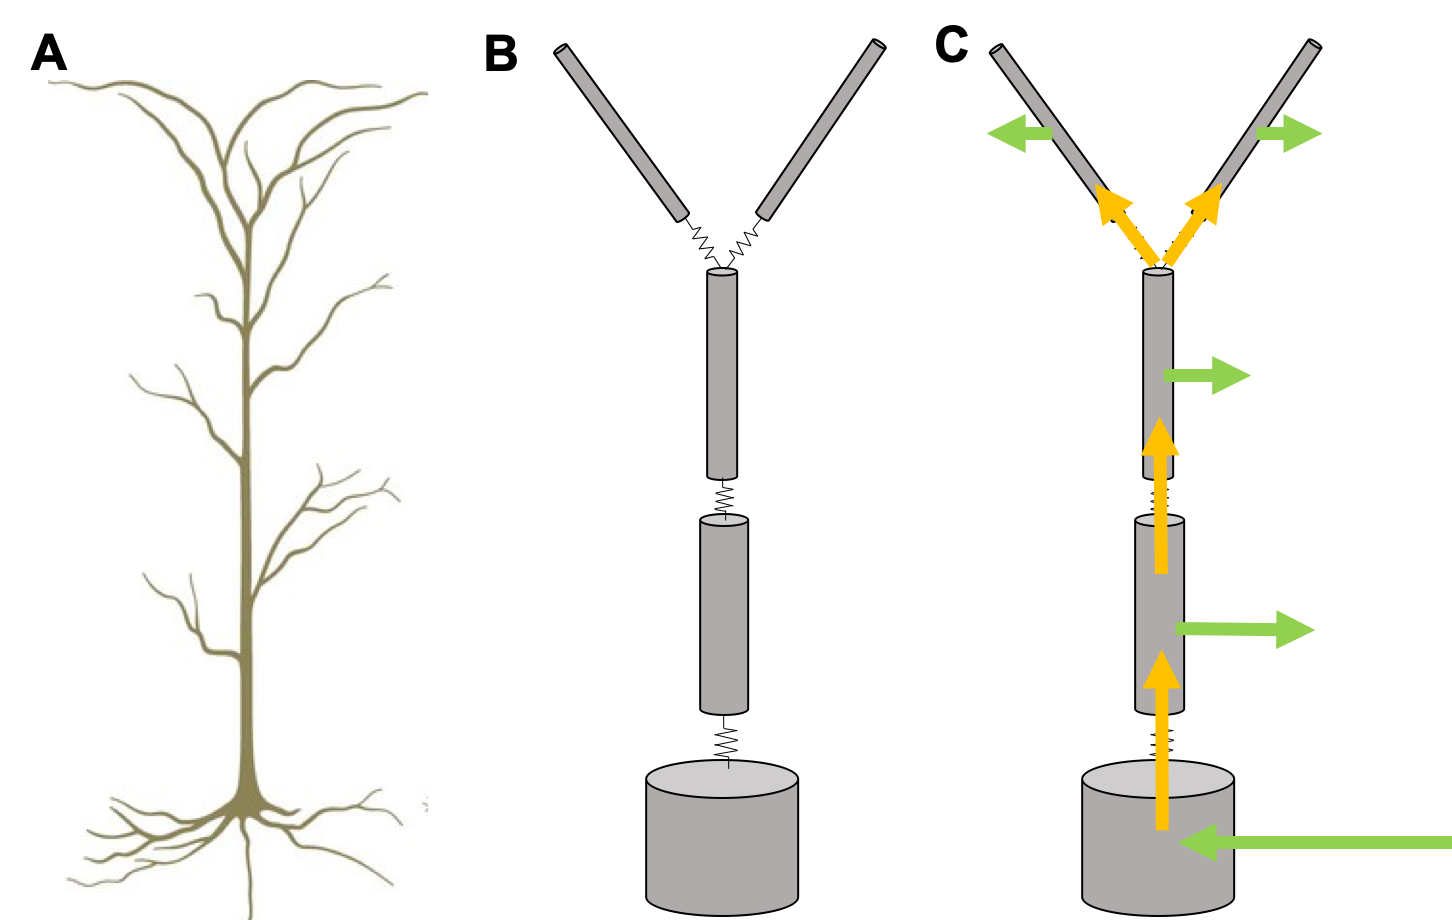
\includegraphics[width=0.6\textwidth]{Figures/Multicomp.png}
\end{center}
\caption{\textbf{Multicompartmental modelling.} 
}
\label{fig:multicomp}
\end{figure}


\subsubsection{Ion channels}
\ghnote{Skriv om HH-formalisme her.}

\subsubsection{Morphology}
\ghnote{Skriv om multicomp her}

\subsection{Cable theory}
\ghnote{Skriv om cable theory her, og noen analytiske tilfeller som hjelper oss aa faa en kjerneforstaaelse.}

\subsection{Point neurons}
\ghnote{skriv om punktmodeller her, problemet med at de ikke gir opphav til ekstracellulare felter, og triks for aa bruke dem likevel.}

\subsection{Constant concentrations approximation}
\ghnote{Skrive om konsentrasjonseffekter. Tror det er bra aa spare Nernst-potensialene til dette delkap. Si noe om at man ofte ikke trenger aa holde styr paa konsentrasjoner pga. homeostatiske mekanismer "bakt inn" i passiv lekkasje.Si noe om hva som skal til for faktisk aa modellere konsentrasjoner uten aa gaa inn i detalj. Referere til rammeverkene som kommer i Kap 6.}
